%!TEX ROOT = ../mainCZ.tex
%\input{./text_cz/mat_a_met/2}

% Úvodní část je věnována historickému pozadí a vývoji modelu SMODERP. Odvození parametrů o kterých se hovoří v kapitole \ref{SM_hist} jsou podrobně popsány v kapitole \ref{Exp_mer}. Použité fyzikální vztahy jsou popsány v kapitole \ref{modelovani}. SOučasná verze modelu z hlediska zpracování vstupních dat, výpočtu a uváděných výstupů je pak v kapitole \ref{vypocet}.



V poslední části manuálu jsou ukázány výsledky modelu \smod a jejich porovnání s původní 1D profilovou verzí na experimentálním povodí Býkovice. \\
\rule{\textwidth}{0.3pt}



\section{Porovnání metod 1D a 2D} \label{porovnani1D2D}

\pozn{tu jsem to prelozil a nejake anglicke verze, takze si nejsem jist jestli je vse ok}

\smod a předchozí 1D profilová verze byli porovnány pomocí výpočtu průtoku a odteklého objemu na erozně narušených profilech. Toto porovnání bylo provedeno na monitorovaném území povodí Býkovice a Hořovickém potoce, území o rozloze 1.5 $km^{2}$. Při výpočtu 1D řešení bylo vybráno 12 reprezentativních profilů. Řešené území i jednotlivé profily vybrané pro 1D výpočet jsou ukázaný na mapě na obrázku~\ref{fig:horany1}. Oba typy řešení byly modelování pro stejnou naměřenou srážku. Průtok v uzávěrovém profilu byl u 1D řešení určen součtem odtoku jednotlivých reprezentativních úseků. Výsledky porovnání jsou ukázány v grafu~\ref{graf:graf_1}. Výsledky odvozené 1D řešení reagují na příčinnou srážku dříve 2D řešení i doba koncentrace je kratší. Při dotoku reaguje 1D řešení na pozdější srážku více než 2D řešení. \pozn{jeste z toho neco vyvodit, jak je 2D super.}


% 1D and 2D approaches which are subject to comparison were designated by a hydrograph and runoff volume in the breach profile. The respective comparison was carried out on two locations in the Czech Republic (Hořanský stream and Býkovický catchment). A system of erosion control measures was implemented in this area. The size of the given area being subject to this research is 1.5 $ km^{2} $. For 1D model are the individual agricultural plots were distinguished by 12 different profiles.

\begin{figure}[t]
\centering
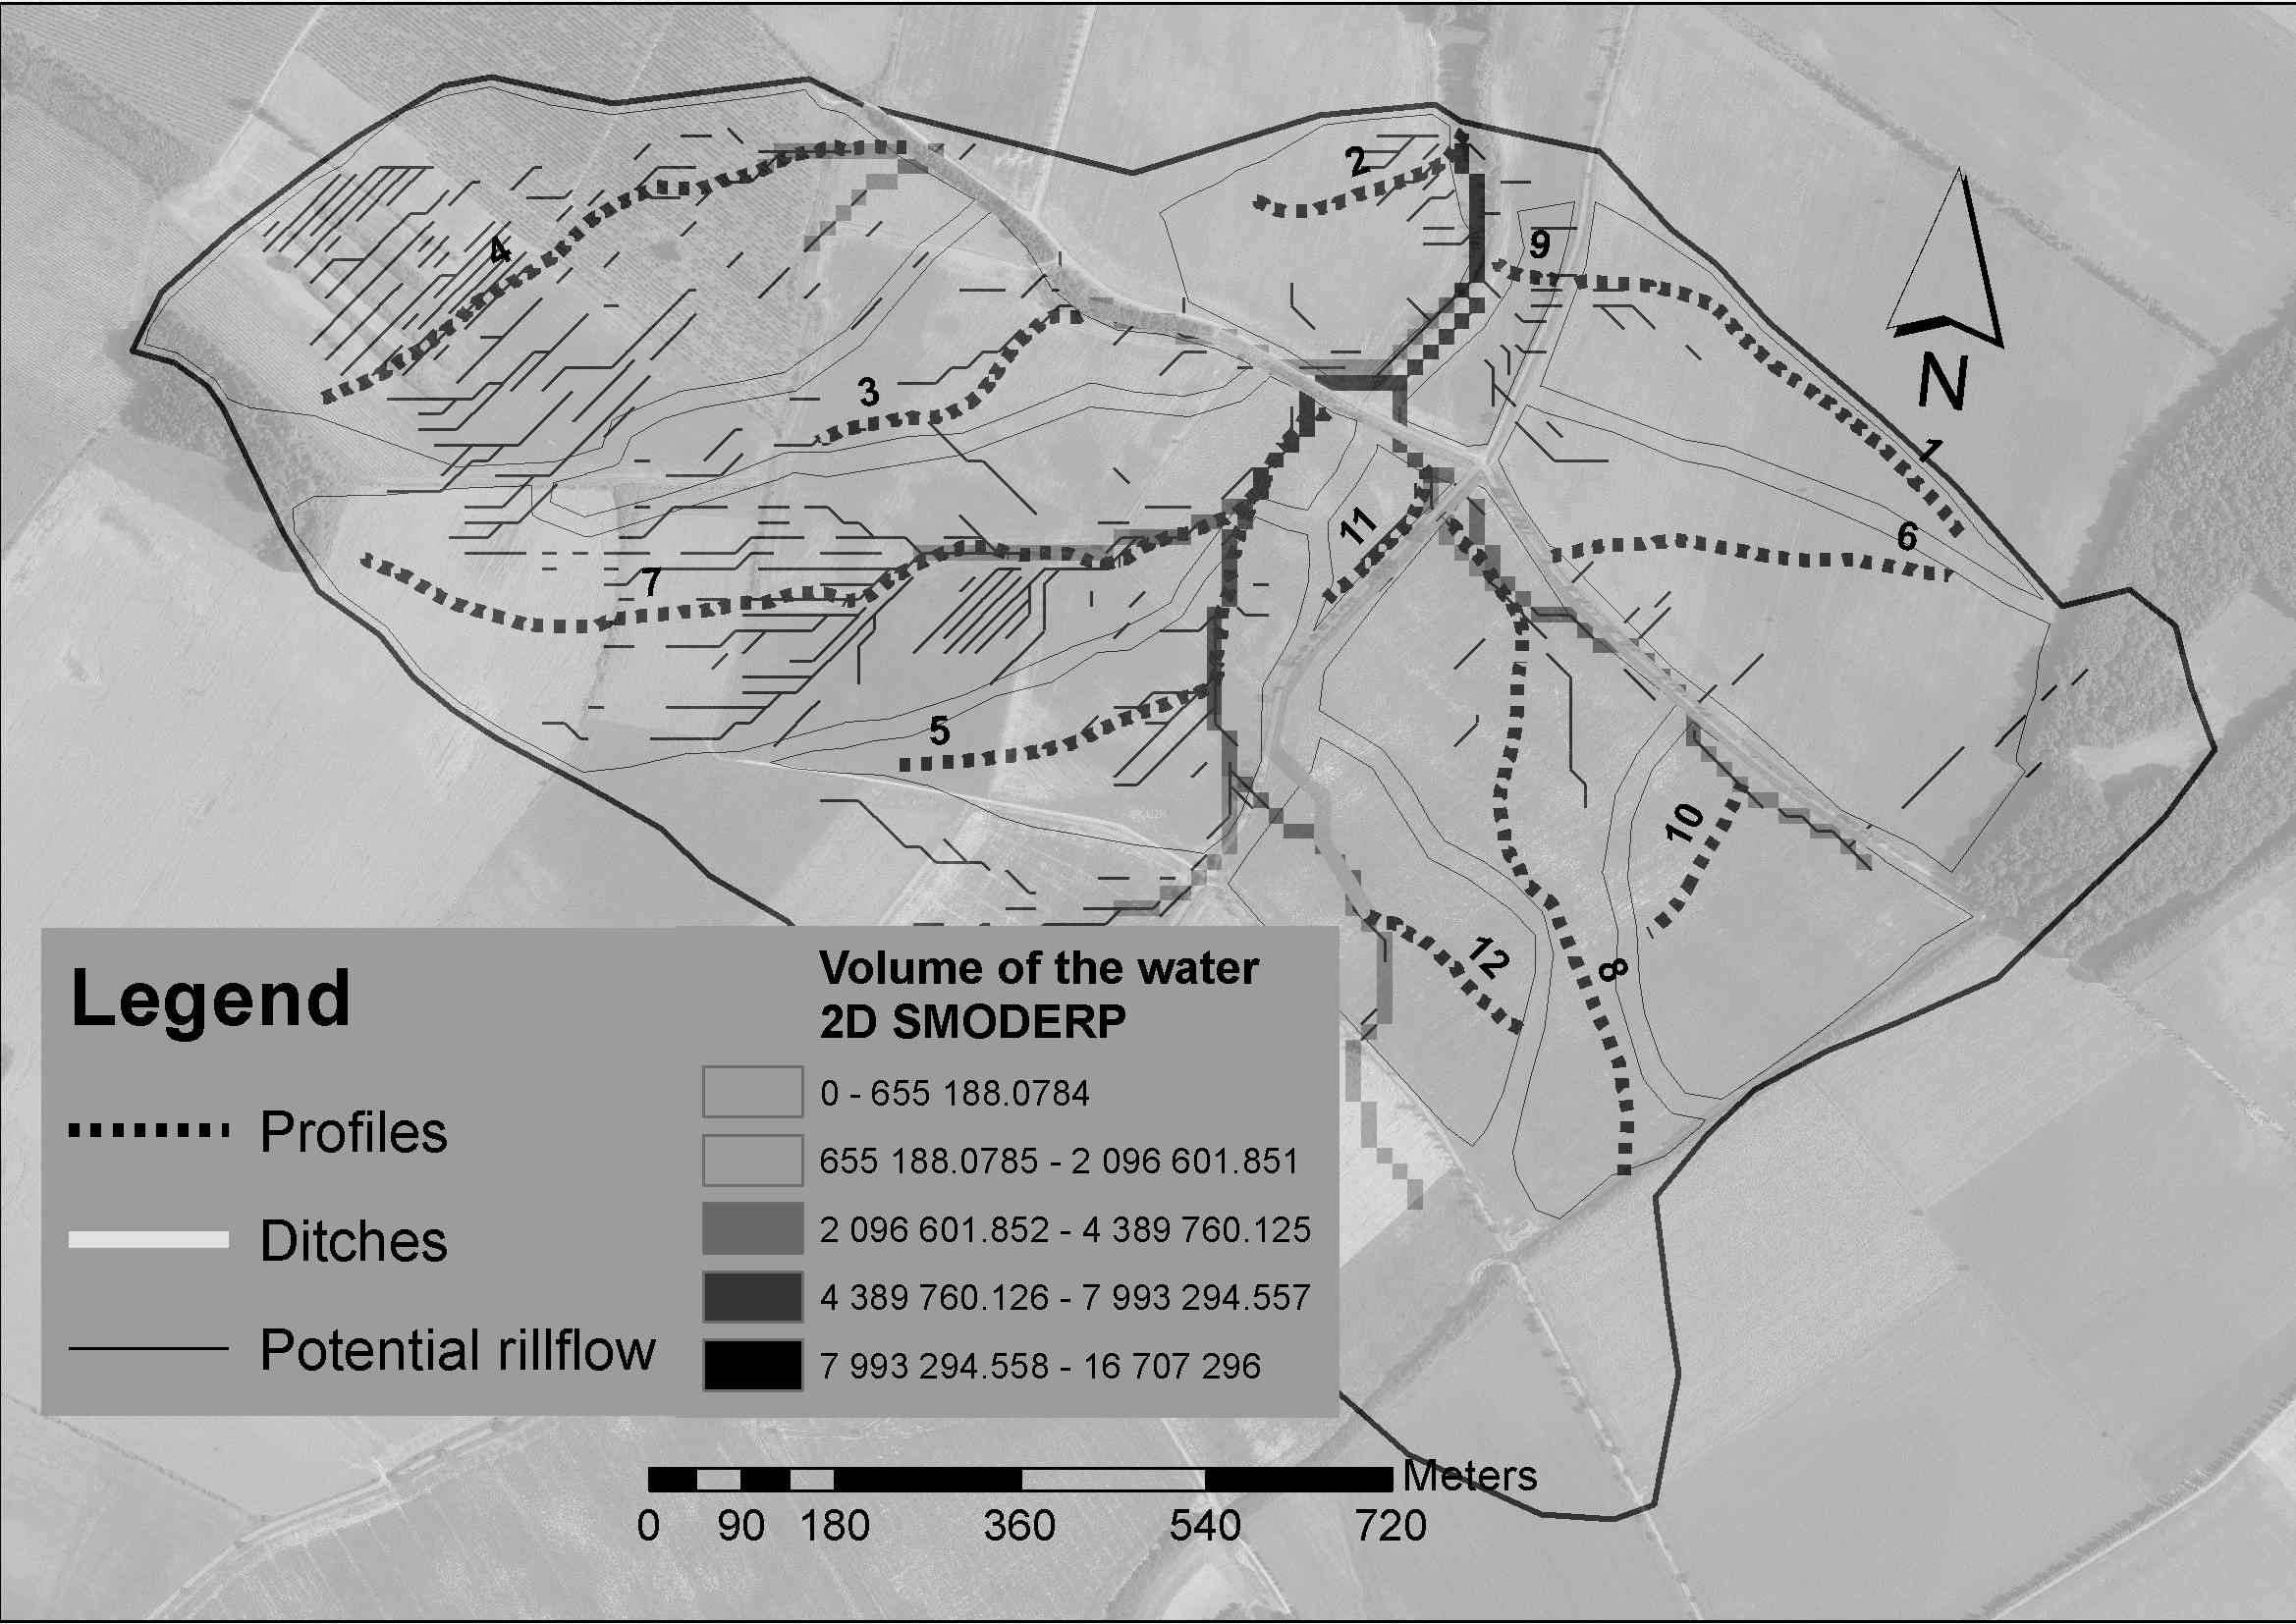
\includegraphics[width=0.6\textwidth]{img/horany_print3.jpg}
\caption{Povodí Býkovice a Hořovický potok. Jednotlivé profily 1D řešení jsou na mapě označené číslem 1-12. Obrázek rovněž ukazuje oblasti rizika vzniku rýh, které sou odvozeny z 2D řešení}
\label{fig:horany1}
\end{figure}%\FloatBarrier
% 
\begin{figure}[t]
\renewcommand{\figurename}{Graf}
\centering
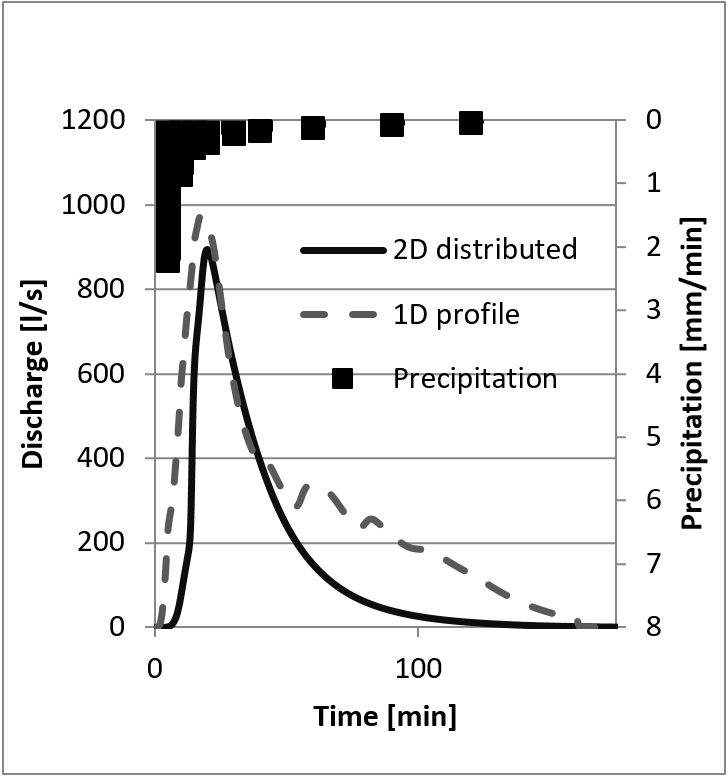
\includegraphics[width=0.6\textwidth]{graph/1D2Dhorany.png}
\caption{Srovnání 1D a 2D řešení modelu \smod - Povodí Býkovice a Hořovický potok}
\label{graf:graf_1}
\end{figure}

\FloatBarrier

% The second location is formed by the independent agricultural plot situated in the Býkovický potok basin (Benešov u Prahy) with a morphologically distinctive lane of concentration runoff. Experimental measurements of erosion processes were carried out on the given plot for a considerable period of time. It is thus possible to compare the final results for the appropriate model with measured values. Six characteristic profiles were created on the given plot (size of ten acres). This number exceeds considerably the amount of profiles which were necessary for the description of the given small area. The number of profiles was appointed in order to make comparisons between 1D and 2D approaches, as well as from the reasons explaining the influence of a large number of profiles on the final characteristics. Standardized field erosion plots were installed and situated on a farmer plot in the surveyed area for monitoring the overland flow and sediment transport. The resulting cooperation between the 1D and 2D approaches was executed during the real rainstorm with measured surface runoff.

% \begin{figure}[ht!]
% \centering
% 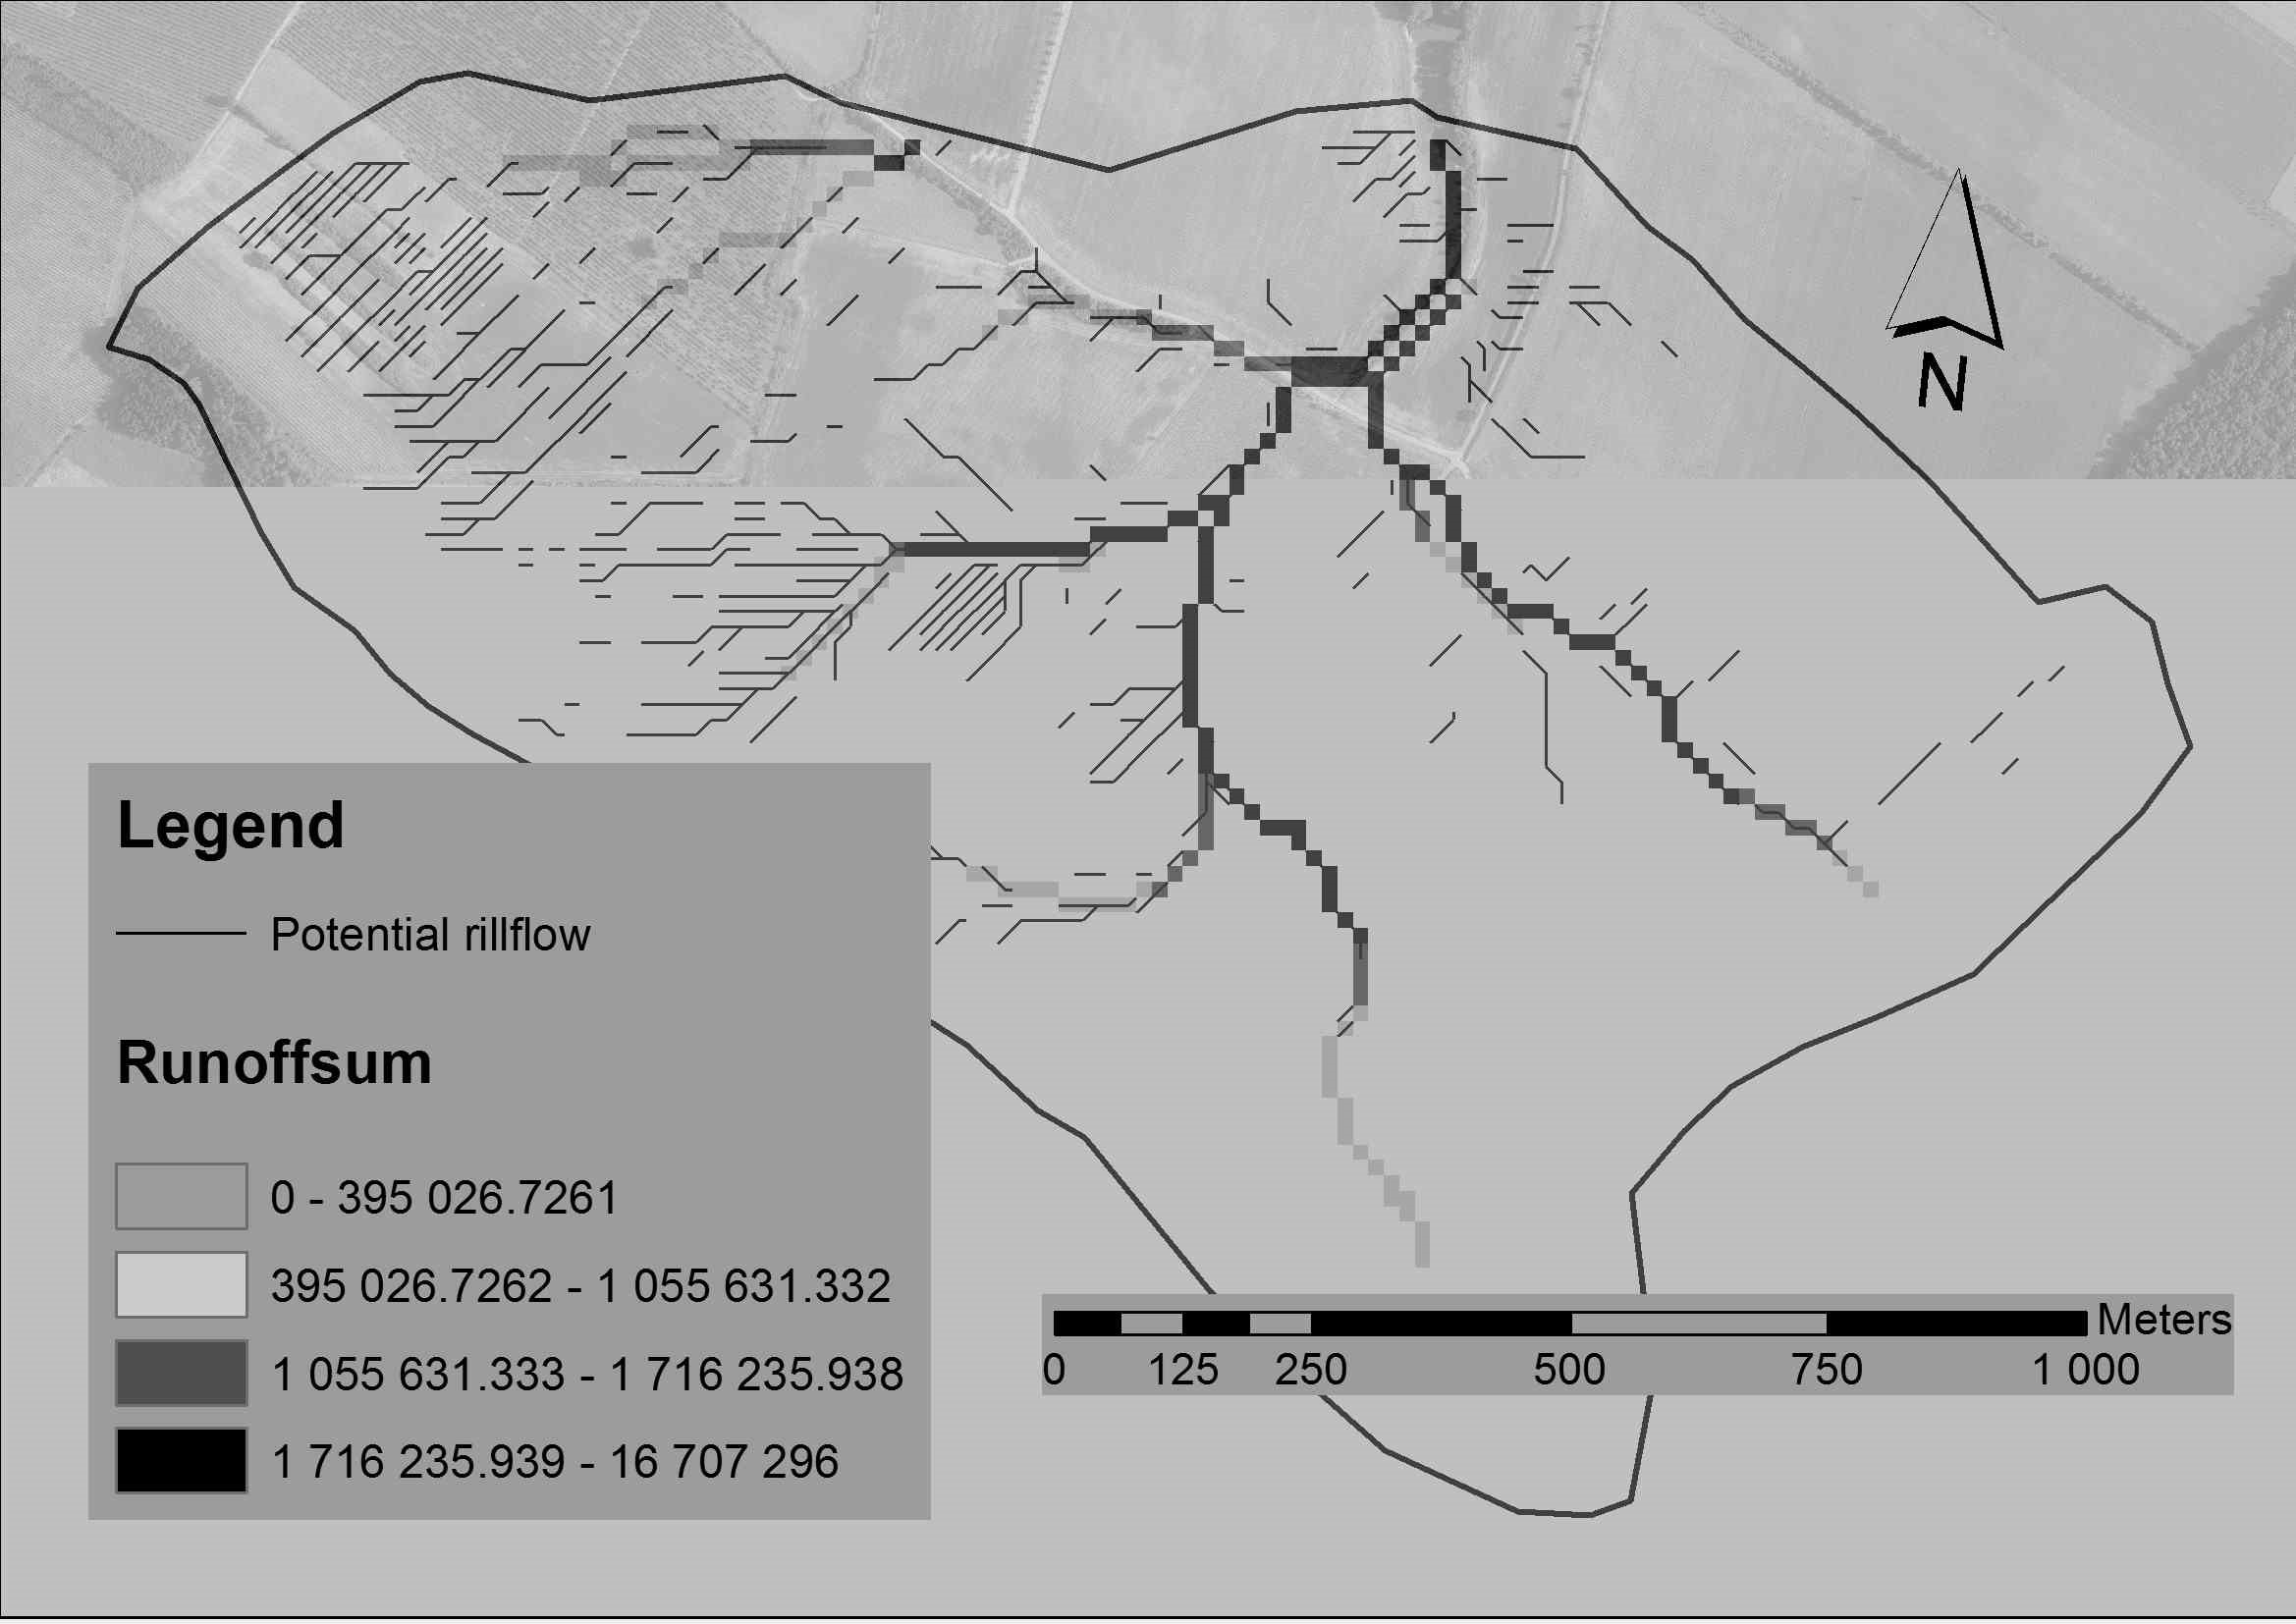
\includegraphics[width=0.8\textwidth]{img/byk.jpg}
% \caption{Profiles and runof concetration - Bykovicky catchment }
% \label{fig:horany2}
% \end{figure}\FloatBarrier
% 
% \begin{figure}[ht!]
% \renewcommand{\figurename}{Graf}
% \centering
% 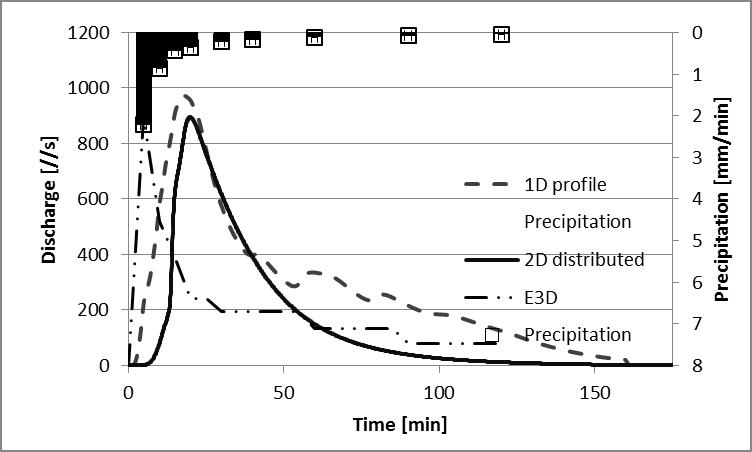
\includegraphics[width=0.8\textwidth]{graph/1D2DByk.jpg}
% \caption{Hydrographs 1D and 2D Smoderp - Bykovicky catchment}
% \label{graf:graf_2}
% \end{figure}\FloatBarrier

% The results based on hydrograph measurements taken from individual profiles in both locations were progressively added to the breach profile (outlet). In order to compare the discharge process, the values of surface level, discharge and a cell of the breach profile were extracted in the 2D model version for testing. The implementation of this process is enabled in the development environment of the particular model.
%\clearpage
%\newpage\null\thispagestyle{empty}\newpage
